\documentclass[french,12pt]{article}

\usepackage{graphicx} % Required for inserting images
\usepackage{subfigure}
\usepackage{float}
\usepackage{tikz}
\usetikzlibrary{positioning}

% Set page size and margins
% Replace `letterpaper' with `a4paper' for UK/EU standard size
\usepackage[letterpaper,top=2cm,bottom=2cm,left=3cm,
right=3cm,marginparwidth=1.75cm]{geometry}
\usepackage{csquotes}

% Useful packages

\usepackage{fix-cm}% to provide smooth tiny font sizes
\usepackage{amsmath,mathtools}
\usepackage{bbm}
\usepackage{amsfonts}
\usepackage{graphicx}
% \usepackage{algpseudocode}
% \usepackage{algorithm}
\usepackage[ruled, lined]{algorithm2e}
\usepackage[colorlinks=true, allcolors=blue]{hyperref}

% Langue
% \usepackage[french]{babel}
\usepackage{babel}
\usepackage[T1]{fontenc}

% Redirection avec la table des matières
\hypersetup{
    colorlinks,
    citecolor=black,
    filecolor=black,
    linkcolor=black,
    urlcolor=black
}

% Pour les scripts
\usepackage{listings}
\usepackage{xcolor}

\definecolor{codegreen}{rgb}{0,0.6,0}
\definecolor{codegray}{rgb}{0.5,0.5,0.5}
\definecolor{codepurple}{rgb}{0.58,0,0.82}
\definecolor{backcolour}{rgb}{0.95,0.95,0.92}

\lstdefinestyle{mystyle}{
    backgroundcolor=\color{backcolour},
    commentstyle=\color{codegreen},
    keywordstyle=\color{magenta},
    numberstyle=\tiny\color{codegray},
    stringstyle=\color{codepurple},
    basicstyle=\ttfamily\footnotesize,
    breakatwhitespace=false,
    breaklines=true,
    captionpos=b,
    keepspaces=true,
    numbers=left,
    numbersep=5pt,
    showspaces=false,
    showstringspaces=false,
    showtabs=false,
    tabsize=2
}

\lstset{style=mystyle}

\title{PFE}
\author{Khaled MEDJKOUH \\ Davidson Lova RAZAFINDRAKOTO}

\begin{document}

\maketitle

\pagebreak

\tableofcontents

\pagebreak

\section{Introduction}

Aujourd'hui, les applications des modèles/algorithmes d'apprentissage machine à base
de réseaux de neurones arrivent à accomplir des tâches variées et de plus 
en plus complexes. Ce sont des modèles paramétriques souvent avec un nombre très 
importants de paramètres à ajuster pendant la période d'entrainement. En fonction des
conditions de l'entrainement du modèles (données d'entrainement, choix d'hypeparamètres),
ces paramètres ne seront pas les mêmes et naturellement la sortie du modèle
sera affecté par cette variabilité. Comme la fonction du modèle est de sortir la bonne
sortie quand on introduit une entrée, il y a un besoin de savoir contrôler cette variabilité
pour avoir une confiance dans le résultat du modèle. Ce travail va tenter de reproduire un 
des méthodes qui tentent à contrôler cette variabilité, proposée dans cet article \cite{Fernndez2022}, 
l'algorithme BNN-ABC-SS.


\subsection{Réseau de neurones \href{https://en.wikipedia.org/wiki/Feedforward_neural_network}{\textit{feedforward}}}

Un réseau de neurones \href{https://en.wikipedia.org/wiki/Feedforward_neural_network}{\textit{feedforward}} est une fonction non linéaire paramétrée.
La fonction prend au niveau de sa couche d'entrée un vecteur d'entrée $x \in \mathcal{X}$, le transforme 
à travers les couches cachées pour enfin sortir un vecteur de sortie $y \in \mathcal{Y}$ à la couche de sortie.

\begin{figure}[H]
    \centerline{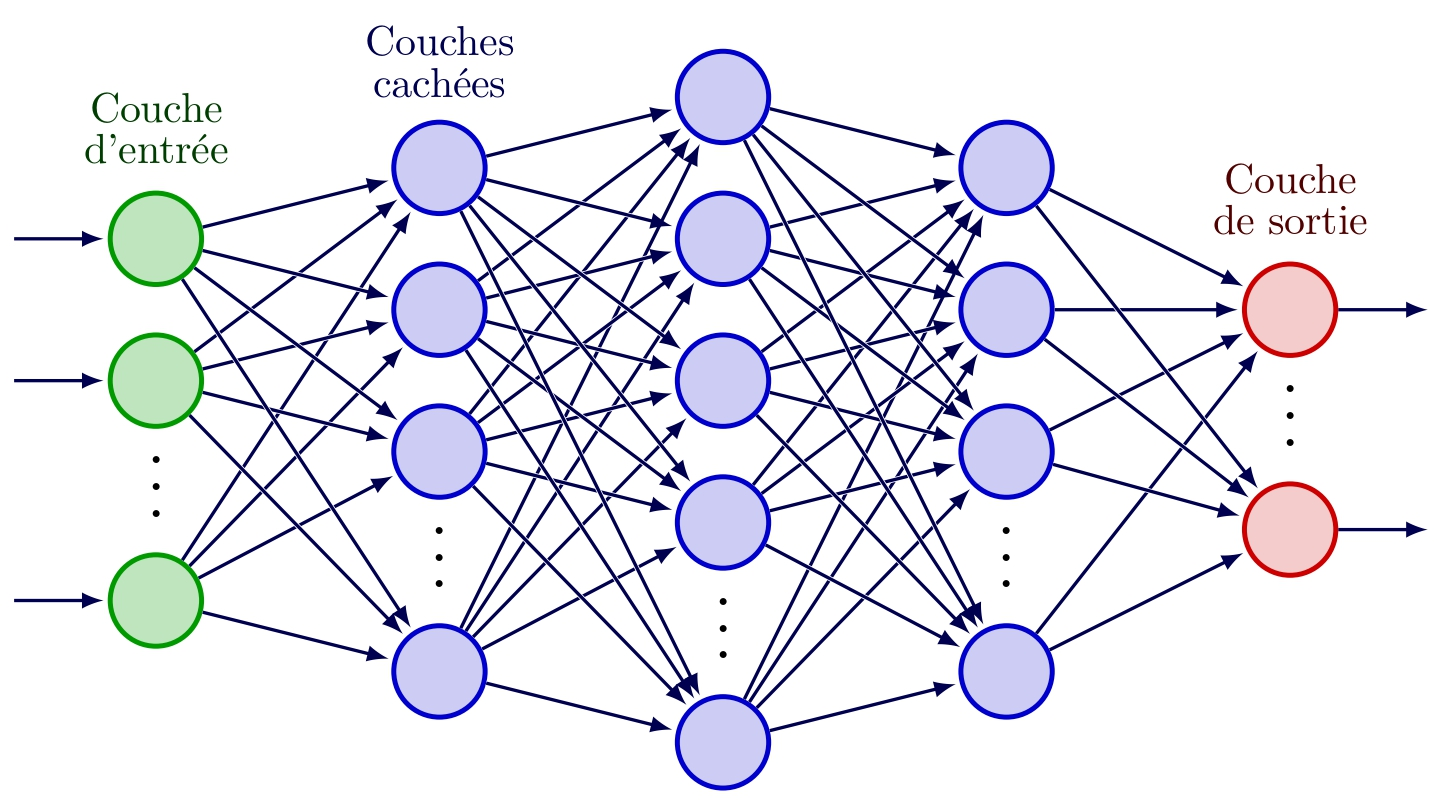
\includegraphics[width = 0.6\textwidth]{FNN/Images/fnn/fnn_page-0001.jpg}}
    \caption{Schéma de réseaux \href{https://en.wikipedia.org/wiki/Feedforward_neural_network}{\textit{feedforward}} \cite{NeetGraph}}
    \label{fig:fnn}
\end{figure}

Pour passer d'une couche à une autre chaque neurone $a^{(j + 1)}_s$ de la couche d'arrivée reçoit une contribution
des neurones $\{a^{(j)}_i\}_{i = 1}^n$ de la couche de départ pondérés par les poids
$\{w^{(j)}_{i,s}\}_{i = 1}^n$. Cette contribution sera biaisé (avec $b^{(j)}_s$) ensuite transformée par une fonction
qu'on appelle $\textit{fonction d'activation}$ noté $\sigma$.

\begin{figure}[H]
    \centerline{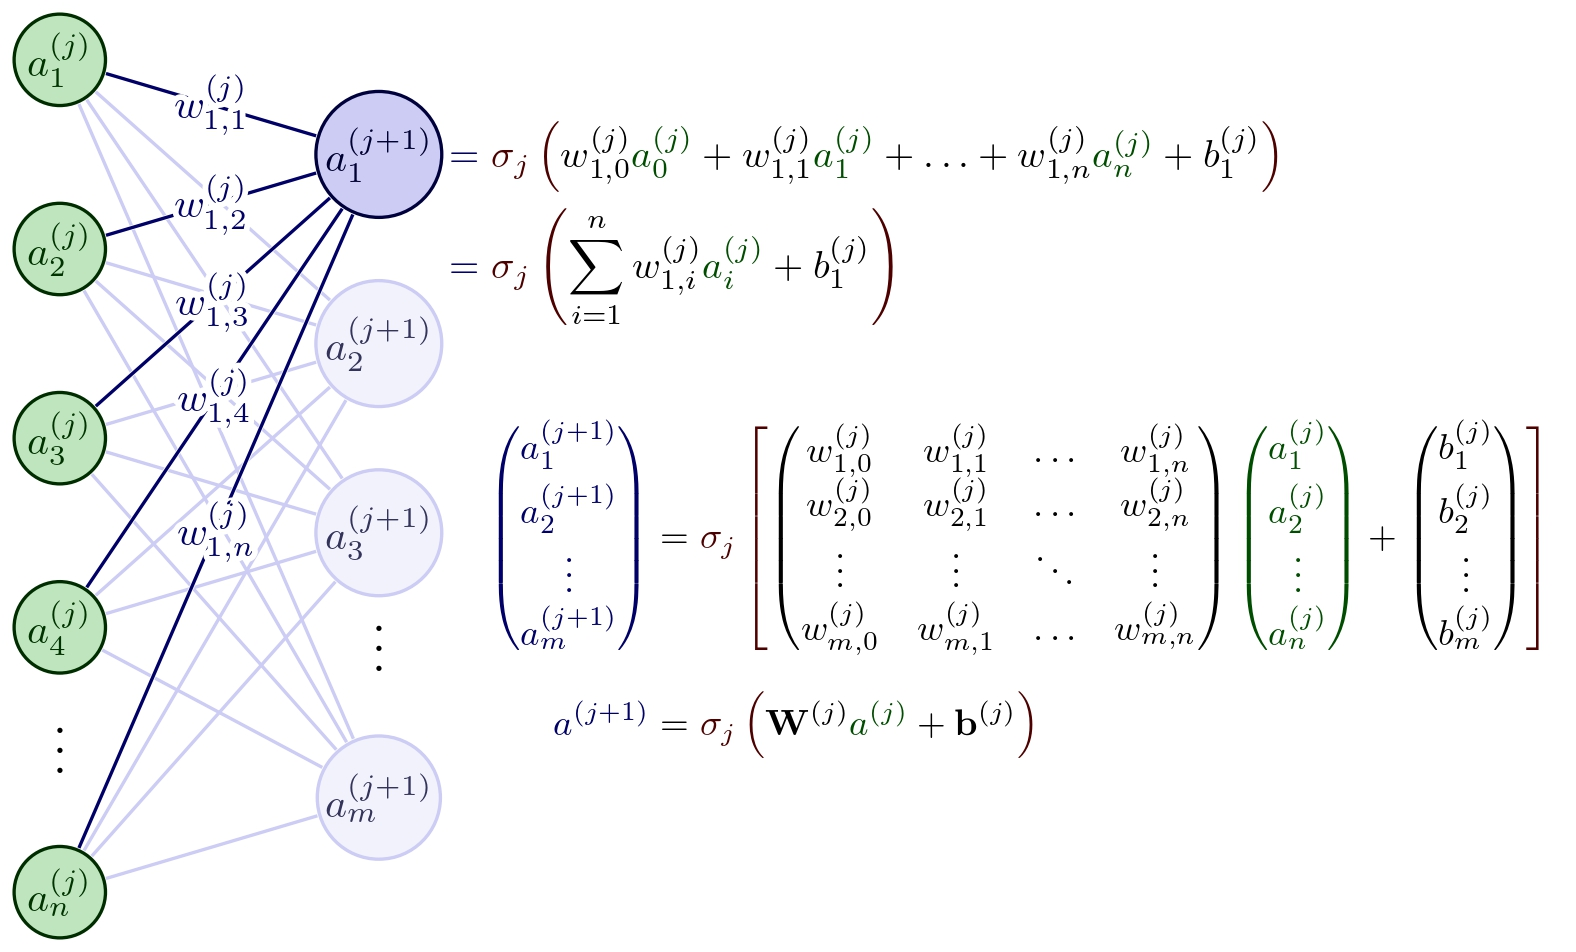
\includegraphics[width = 0.75\textwidth]{FNN/Images/fnnDetails/fnnDetails_page-0001.jpg}}
    \caption{Passage d'une couche à la prochaine couche \cite{NeetGraph}}
    \label{fig:fnnDetails}
\end{figure}

Pour la couche de sortie, en fonction des applications on choisit une fonction d'activation $\sigma'$
différente de $\sigma$ (par exemple l'identité pour la régression et softmax pour la classification).

\subsection{Source d'incertitudes dans un réseaux de neurones}

On modélise le réseau de neurones \href{https://en.wikipedia.org/wiki/Feedforward_neural_network}{\textit{feedforward}} comme la fonction non linéaire

$$f : (x, \theta) \in \mathcal{X} \times \Theta \mapsto f(x, \theta) \in \mathcal{Y}$$

où

\begin{itemize}
    \item $\mathcal{X} \subset \mathbb{R}^{n_e}$, l'espace des variables d'entrée
    \item $\mathcal{Y} \subset \mathbb{R}^{n_s}$, l'espace des variables de sortie
    \item $\Theta \subset \mathbb{R}^{n_p}$ , l'espace des paramètres
\end{itemize}

On se donne maintenant une base de données d'entrainement
$D = \{ (x_i, y_i)\}_{i = 1}^N \in (\mathcal{X} \times \mathcal{Y})^N$.

\subsubsection{Acquisition des données}

Si on prend comme données d'entrée $x$ une mesure d'une quantité réelle $\tilde{x}$.

Il y a une variabilité sur la mesure en fonction des circonstances
et conditions $\omega \in \Omega$ où la mesure a été effectué en 
plus de la précision de l'appareil de mesure.

La sortie $y$ peut aussi subir des erreurs de labélisation
(pour le cas d'une tâche de classification) ou aussi de mesure si c'est 
une quantité mesurée ou issue d'une quantité mesurée.

En somme on a une incertitude sur l'entrée $x | \omega \sim p_{x | \omega}$
et $y | \omega \sim p_{y | \omega}$.

S'ajoute à cela, l'incertitude sur $x$ qui peut se propager sur $y$.

\subsubsection{Structure du modèle}

Les paramètres $\theta$ et donc l'espace $\Theta$ est variable en fonction du choix de modèle $s$.

On a $\theta | D,s \sim p_{\theta | D, s}$

\subsection{Prédiction}

La prédiction faite à partir d'un réseau entrainé subit alors les incertitudes venant
de ces sources. La distribution de la prédiction $y^*$ sachant une entrée $x^*$ est donné par

$$ p(y^* | x^*, D) = \int_{\Theta} \underbrace{p(y^* | x^*, \theta)}_{\text{Données}} \underbrace{p(\theta  | D)}_{\text{Modèle}} d \theta$$

\subsubsection{Incertitude aléatoire}

L'incertitude dite aléatoire est due à la variabilité innée aux données d'entrainement
du modèle. Elle affecte la partie $p(y^* | x^*, \theta)$ de la tâche de prédiction.

\subsubsection{Incertitude épistémique}

L'incertitude épistémique affecte la partie $p(\theta  | D)$ de la tâche de prédiction,
elle est due :

\begin{itemize}
    \item à la complexité du modèle,
    \item aux erreurs durant la phase d'entrainement,
    \item à la manque d'information à cause de données manquantes
          ou la capacité de représentation des données d'entrainement.
\end{itemize}

\pagebreak

\section{Réseau de neurones bayésiens (BNN)}

% + Présentation de réseaux de neurones bayésiens

Les réseaux de neurones bayésiens sont des réseaux de neurones
dont les paramètres ($\theta = (w, b)$) sont, non pas des quantités déterministes (comme
dans le cas d'un réseau classique) mais des distributions de probabilité.

À l'initialisation, les paramètres suivent une loi a priori $p(\theta)$,
et l'entrainement consiste à évaluer l'a posteriori de cette loi conditionnée
aux données d'entrainement $p(\theta | D)$.

Cette méthode permet de tenir compte de l'incertitude sur le modèle utilisé
avec une structure donnée, car ici, il s'agit d'évaluer 
une famille de modèles au lieu d'un seul.

% + Donner son interet dans la résolution du problème précédent

% + Donner les méthodes d'entrainement d'un tel réseaux
Cependant, à cause de la taille et de la complexité de ces modèles
on ne dispose pas, dans le cas général, d'une formule analytique pour 
calculer cette distribution a posteriori. Des méthodes numériques
ont été développés pour calculer une approximation de cette distribution a posteriori.

Parmis ces méthodes on trouve :
\begin{itemize}
    \item Méthodes variationnelles
    \item Méthodes par échantillonnage ou
          Monte-Carlo (qu'on va voir dans la suite)
    \item Méthodes de Laplace
\end{itemize}


\subsection{Méthodes variationnelles}

Ici on approche $p(\theta | D)$ par une famille de distribution
paramétrique $\{q^{\gamma}(\theta)\}_{\gamma}$ (souvent des gaussiennes).
Le but est de choisir $\gamma$ qui rapproche $q^{\gamma}(\theta)$
le plus de $p(\theta | D)$ au sens de la divergence de Kullback-Leibler :

$$KL(q||p) = \mathbb{E}_q \left[\log \frac{q^{\gamma}(\theta)}{p(\theta | D)}\right]$$

Comme on ne connaît pas $p(\theta | D)$, on utilise l'ELBO (\textit{evidence lower bound})
qui est égal à la divergence à une constante près

$$L =\mathbb{E}_q \left[\log \frac{p(y | D, \theta)}{q^{\gamma}(\theta)}\right]$$

(on a en effet $KL(q||p) = -L +  \log p(y| D)$)

On résout ici un problème d'optimisation.

\subsection{Méthode de Laplace}

$\hat{\theta}$ l'estimateur de maximum d'a priori.

$$\log p(\theta | D) \approx \log p(\hat{\theta} | D)
    + \frac{1}{2} (\theta - \hat{\theta})^T (H + \tau I)
    (\theta - \hat{\theta})$$

$$p(\theta | D) \sim \mathcal{N}(\hat{\theta}, (H + \tau I)^{-1})$$

\subsection{Méthodes par échantillonage ou \href{https://en.wikipedia.org/wiki/Monte_Carlo_method}{Monte Carlo}}

La formule de Bayes nous donne

$$p(\theta | D) = \frac{p(D | \theta) }{p(D)}p(\theta)$$

\begin{itemize}
    \item $p(D | \theta)$ la vraisemblance des données $D$ sachant le paramètre $\theta$,
    \item $p(\theta)$ la distribution a priori de $\theta$,
    \item $p(D)$ la distribution des données d'entrainement.
\end{itemize}

Il s'agit de faire des tirages de $\theta$ pour évaluer ces quantités.

\pagebreak

\section{Algorithme BNN-ABC-SS}

\subsection{ABC (\href{https://en.wikipedia.org/wiki/Approximate_Bayesian_computation}{\textit{Approximate Bayesian Computation}})}

La méthode ABC consiste à evaluer $p(\theta | D)$ sans évaluer
la vraisemblance qui peut s'avérer couteux.

Posons $\hat{y} = f(x, \theta)$ la sortie d'une évaluation de $x$ par
réseaux de neurones $f$ avec paramètre $\theta$.

La formule de Bayes nous donne

$$ p(\theta, \hat{y} | D) \propto p(D | \hat{y}, \theta) p(\hat{y} | \theta)
    p(\theta)$$

Pour simuler selon la distribution du second membre, on applique
l'algorithme de rejet.

\begin{itemize}
    \item On tire $\theta \sim p(\theta)$
    \item On evalue $\hat{y} = f(x , \theta) \sim p(\hat{y} | \theta)$
    \item On accepte le $\theta$ si et seulement si $\hat{y} = y$
\end{itemize}

Comme $\hat{y}$ est une quantité réelle (a priori à distribution continue),
obtenir exactement $\hat{y} = y$ est une condition trop forte
pour être atteinte (en un temps raisonnable).

On introduit alors une tolérance $\epsilon$, on remplace $\hat{y} = y$
par $|\hat{y} - y| < \epsilon$.

On remarque que plus $\epsilon$ est petit, plus on se rapproche de la condition $\hat{y} = y$,
et donc le mieux notre approximation sera.

On note $p_{\epsilon} (\theta, \hat{y} | D)$ la distribution issue
du tirage précédent, et qui approche $p(\theta, \hat{y} |D)$, on a

$$p_{\epsilon} (\theta , \hat{y} | D) \propto \mathbbm{1}_{\mathcal{N}_{\epsilon}(D)} (\hat{y}) p(\hat{y} | \theta)
    p(\theta) $$

où $$\mathcal{N}_{\epsilon}(D) = \{\hat{y} \in \mathcal{Y}, \rho(\eta(\hat{y}), \eta(y)) \leq \epsilon\}$$


où $\eta$ est une statistique qui caractérise une distribution
(par exemple les moments ou les quantiles) et $\rho$ est une mesure de dissimilarité.

En intégrant des deux côtés par $\hat{y}$ on obtient notre approximation de $p(\theta | D)$

$$p_{\epsilon}( \theta | D) = \int_{\mathcal{Y}} p_{\epsilon}( \theta , \hat{y}| D) d \hat{y} \propto \int_{\mathcal{Y}} \mathbb{I}_{\mathcal{N}_\epsilon (D)} (\hat{y}) p( \hat{y}| \theta) p( \theta) d \hat{y}$$

$$ = p( \theta) \int_{\mathcal{Y}} \mathbb{I}_{\mathcal{N}_\epsilon (D)} (\hat{y})  p( \hat{y}| \theta) d \hat{y} = \mathbb{P} (\hat{y} \in \mathcal{N}_{\epsilon} (D)| \theta) p( \theta)$$

Cependant lors de l'algorithme de rejet, tirer les $\theta$ de manière générique donne trop rarement des $\hat{y}$ qui tombent dans $\mathcal{N}_{\epsilon} (D)$
ce qui fait que l'approximation est prend beaucoup de temps à converger. On utilise alors SS (Subset Simulation)
pour faire des tirages plus fins.

\subsection{SS (\href{https://en.wikipedia.org/wiki/Subset_simulation}{\textit{Subset Simulation}})}

Soient $\epsilon_1 > \epsilon_2 > ... >\epsilon_m = \epsilon$ des seuils.

Il est clair que $\mathcal{N}_{\epsilon_m} (D)\subset \mathcal{N}_{\epsilon_{m - 1}} (D)
    \subset ... \subset \mathcal{N}_{\epsilon_{2}} (D) \subset \mathcal{N}_{\epsilon_{1}} (D)$.

De plus et en conséquence, $\bigcap_{j = 1}^m \mathcal{N}_{\epsilon_j} = \mathcal{N}_{\epsilon_m} = \mathcal{N}_{\epsilon} $, ce qui nous donne

$$ \mathbb{P} \left(\hat{y} \in \mathcal{N}_{\epsilon} (D)| \theta \right) = \mathbb{P} \left(\hat{y} \in \bigcap_{j = 1}^m \mathcal{N}_{\epsilon_j} (D)| \theta\right)$$

$$= \mathbb{P} \left(\hat{y} \in \mathcal{N}_{\epsilon_1} (D)| \theta\right)
    \prod_{j = 2}^{m} \mathbb{P} \left(\hat{y} \in \mathcal{N}_{\epsilon_j} (D)|\hat{y} \in \mathcal{N}_{\epsilon_{j - 1}} (D), \theta\right)$$


L'idée de la SS, est de faire des tirages itératifs de plus en plus fins.

Initialement on tire de manière générique avec un $\epsilon_1$ grand.

À chaque itération, on tire à partir (conditionnés) des tirages précédents avec une tolérance $\epsilon_i$ plus petite.

Après $n$ itérations, on aura tiré avec $\epsilon_m$ beaucoup plus petit que $\epsilon_0$.

Cette méthode exploite la décomposition d'une probabilité d'un ordre très petit
en un produit de probabilité d'un ordre assez grand pour être calculable en un temps raisonnable.



\subsection{Pseudo - Code}

%% This declares a command \Comment
%% The argument will be surrounded by /* ... */
\SetKwComment{Comment}{/* }{ */}

\begin{algorithm}
    \caption{Pseudo code BNN - ABC - SS}\label{alg:one}
    \Entree{$N \in \mathbb{N}^*$ : le nombre de tirages à chaque itération
        \linebreak $l_{\text{max}}\in \mathbb{N}^{*}$ : le nombre d'itérations maximaux
        \linebreak $P_0$ la proportion de nos tirages qu'on grade pour générer à la prochaine itération
        \linebreak $\epsilon$ : la tolérance finale
        \linebreak $x$ : la variable d'entrée
        \linebreak $y$ : la variable de sortie
    }
    \Sortie{$\left[\theta_1^{(n)}, ...,\theta_N^{(n)} \right]$}

    $NP_0 \gets N * p_0$\;

    $iP_0 \gets p_0^{-1}$\;

    $\left[\theta_1^{(0)}, ..., \theta_N^{(0)}\right]$, $N$ tirage de $\theta \sim p(\theta)$;

    $\left[\hat{y}_1^{(0)}, ..., \hat{y}_1^{(0)}\right] \gets \left[f(x, \theta_1^{(0)}), ..., f(x, \theta_N^{(0)})\right]$;

    $\left[\gamma_1^{(0)},..., \gamma_1^{(0)} \right] \gets \left[\rho(\eta(y), \eta(\hat{y}_1^{(0)})), ..., \rho(\eta(y), \eta(\hat{y}_N^{(0)}))\right]$;


    \Pour{$j \in \{1,..., l_{max}\}$}{

    On ordonne $\left[\gamma_1^{(j-1)},..., \gamma_1^{(j-1)} \right]$ dans l'ordre croissant;

    On réordonne $\left[\theta_1^{(j-1) }, ..., \theta_N^{(j-1)}\right]$ dans cet ordre;

    $\epsilon_j \gets \gamma_{NP_0}^{(j-1)}$ (ou $\frac{1}{2} (\gamma_{NP_0}^{(j-1)} + \gamma_{NP_0 + 1}^{(j-1)})$);

    \Pour{$k \in \{1,..., NP_0\}$}{
    On choisit une graine $\theta_k^{(j-1), 1} = \theta_k^{(j-1)}$ tel que $\hat{y}_k^{(j-1)} \in \mathcal{N}_{\epsilon_j} (D)$

    On génère $iP_0$ états d'une chaine de Markov de $\theta$ tel que $\hat{y}\in \mathcal{N}_{\epsilon_j} (D)$ :

    $\left[ \theta_k^{(j-1), 1}, ..., \theta_k^{(j-1), iP_0} \right]$ et avec ça $\left[\gamma_k^{(j-1), 1},..., \gamma_k^{(j-1), iP_0} \right]$
    }

    $[\theta_1^{(j)},..., \theta_N^{(j)}] \gets [\theta_k^{(j-1), l}, k \in \{1, ..., NP_0\}, l \in \{1, ..., iP_0\}]$

    $[\gamma_1^{(j)},..., \gamma_N^{(j)}] \gets [\gamma_k^{(j-1), l}, k \in \{1, ..., NP_0\}, l \in \{1, ..., iP_0\}]$



    \Si{$\epsilon_j \leq \epsilon$}
    {
        Fin de l'algorithme;
    }

    }
\end{algorithm}

% + A voir si on rajoute ou pas

Pour la génération des chaines de Markov dans l'espace $\mathcal{N}_{\epsilon_{j}} (D)$, On utilise l'algorithme
'Modified Monte Carlo' \cite{Chiachio2014, Modified_MCMC}.

L'algorithme de MCMC \cite{Andrieu2003} appliquées à notre problème s'écrit se déroule comme suit.

On se donne une distribution de proposition $q(.|.)$ et au niveau $j$, à l'étape $n$ de la chaine :

\begin{itemize}
    \item On génère $\theta' \sim q(\theta | \theta)$ et $y' \sim p(x | \theta')$
    \item On accepte $(\theta', x')$ en tant que $(\theta^{(n)}, x^{(n)})$ avec une probabilité :

          $\alpha = \min \left\{ 1, \frac{p(\theta') q(\theta^{(n - 1)} | \theta')}{p(\theta^{(n - 1)}) q(\theta' | \theta^{(n-1)})}\right\}\mathbbm{1}_{\mathcal{N}_{\epsilon_j}} (x')$

    \item Sinon $(\theta^{(n)}, x^{(n)}) = (\theta^{(n-1)}, x^{(n-1)})$
\end{itemize}


Dans les exemples qu'on va prendre après, on a pris
\begin{itemize}
    \item $p(\theta)$ est la densité de la distribution $\mathcal{N}(0, \sigma_0)$
    \item $q(. | b)$ est celle de $ \mathcal{N}(b, \sigma_j)$
\end{itemize}



\pagebreak
\section{Réalisation}
% \footcite{BNN_ABC_SS_main}.
On se donne une base de données à étudier avec une comparaison avec des méthodes déjà existante \cite{Chiachio2014,Fernndez2022,Uncertainty_Deep}
Ici on propose de reproduire un résultat vu dans l'article \cite{Fernndez2022}.

\subsection{Cosinus perturbé}

Les données d'entrainement $D = \{x_i , y(x_i)\}_{i = 1}^{200}$, avec $(x_i)_{i = 1}^N$
une discrétisation uniforme de $[-3, 3]$ et $y(x) = \cos(x) + \zeta$ où $\zeta \sim \mathcal{N}(0, 0.1)$.

Les paramètres de l'algorithme $N : 5000$, $l_{max} : 6$, $P_0 : 0.2$ et $\epsilon : 0.1$.

Le réseau de neurones pris ici a une couche d'entrée, une couche cachée à deux cellules et une couche de sortie ce qui
fait 7 paramètres avec la fonction sigmoïde comme fonction d'activation. La mesure de dissimilarité
choisi est la MSE (\href{https://en.wikipedia.org/wiki/Mean_squared_error}{\textit{Mean Squared Error}}).

\begin{figure}[H]
    \centering
    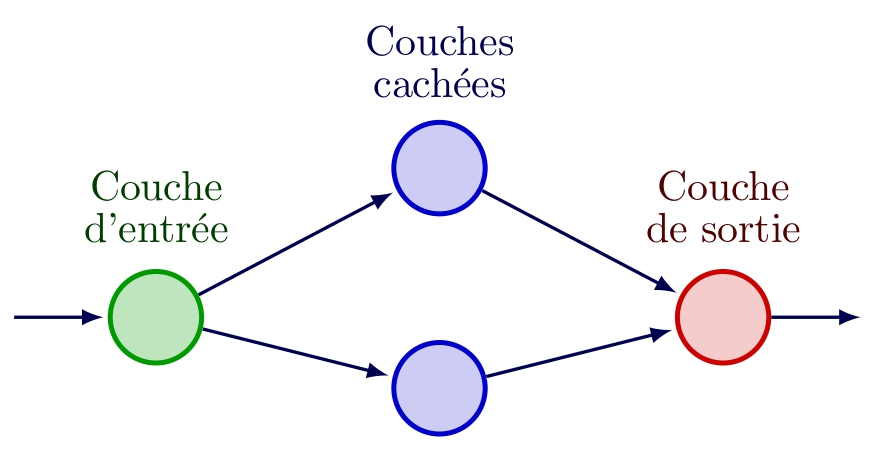
\includegraphics[width = 0.4\textwidth]{FNN/Images/fnnCos/fnnCos_page-0001.jpg}
    \caption[short]{Réseau de neurones pour la fonction $\cos$}
\end{figure}


\begin{figure}[H]
    \centering
    \subfigure[listentry][Données d'entrainement]{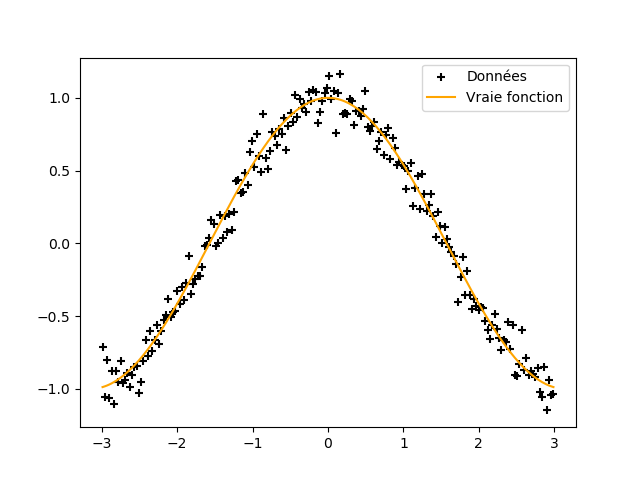
\includegraphics[width = 0.48\textwidth]{../plots/CosPlot.png}}
    \subfigure[listentry][Résultat]{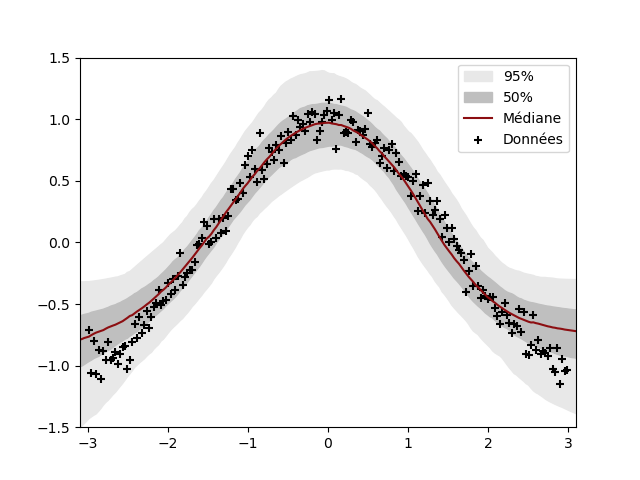
\includegraphics[width = 0.48\textwidth]{../plots/plotCosRes2-11-04-2023_08-47-51.png}}
    \caption[short]{Résultat de l'algorithme BNN-ABC-SS}
\end{figure}

\begin{figure}[H]
    \centering
    \subfigure[$w^{(1)}_{1,1}$]{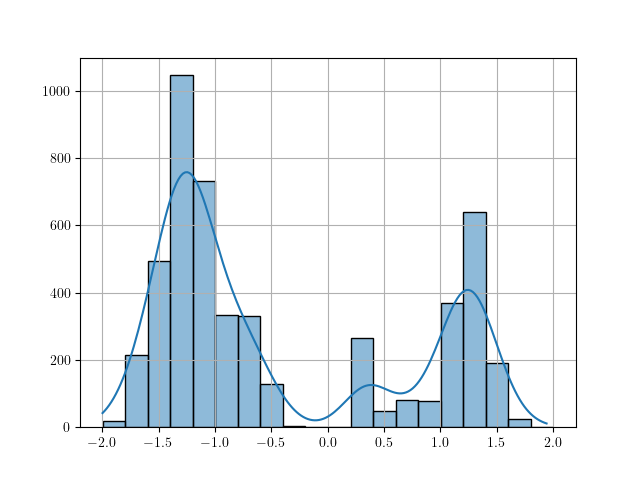
\includegraphics[width = 0.3\textwidth]{../plots/plotWeight-11-04-2023_08-47-51--0.png}}
    \subfigure[$w^{(1)}_{1,2}$]{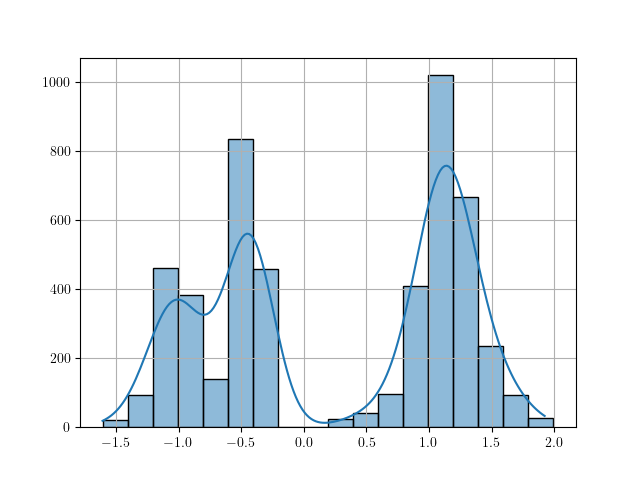
\includegraphics[width = 0.3\textwidth]{../plots/plotWeight-11-04-2023_08-47-51--1.png}}
    \subfigure[$b^{(1)}_{1}$]{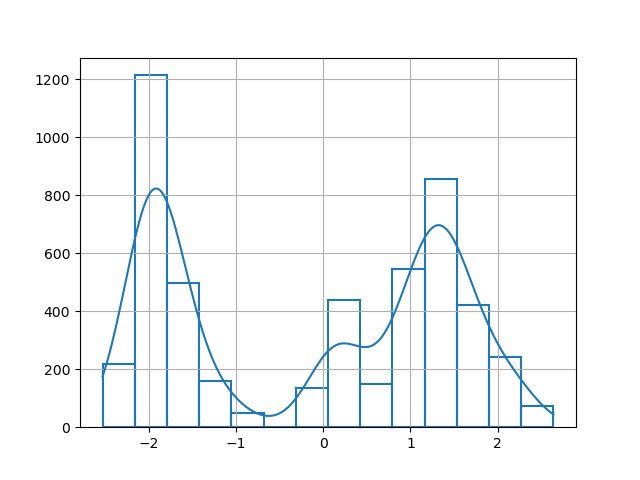
\includegraphics[width = 0.3\textwidth]{../plots/plotWeight-11-04-2023_08-47-51--2.png}}
    \caption[short]{Exemple de distribution a posteriori des poids et biais}
\end{figure}


\begin{figure}[H]
\centering
\begin{tikzpicture}
    \node (img) {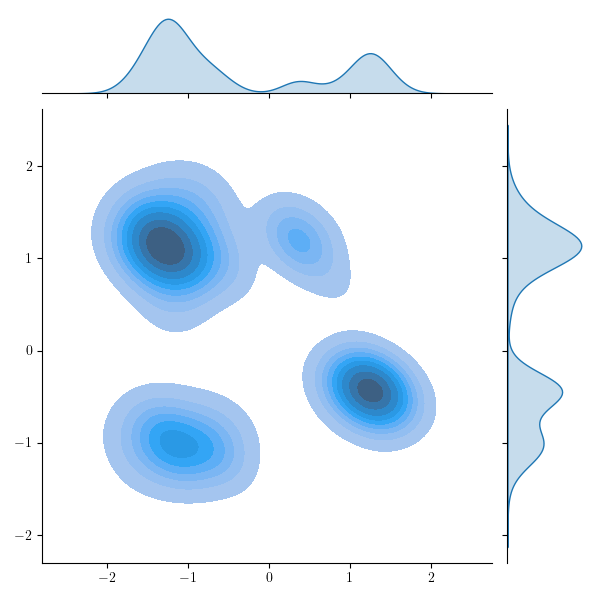
\includegraphics[width = 0.6\textwidth]{../plots/plotWeigthJoint-11-04-2023_08-47-51--0&1.png}};
    \node[below=of img, node distance=0cm, yshift=1cm] {$w^{(1)}_{1,1}$};
    \node[left=of img, node distance=0cm, rotate=90, anchor=center,yshift=-0.7cm] {$w^{(1)}_{1,2}$};
\end{tikzpicture}
\caption{Distribution a posteriori de $w^{(1)}_{1,1}$ et $w^{(1)}_{1,2}$}

\end{figure}

\subsection{Sinus perturbé}


Les données d'entrainement $D = \{x_i , y(x_i)\}_{i = 1}^{100}$, avec $(x_i)_{i = 1}^N$
une discrétisation uniforme de $[-0.5, 0.5]$ et $y(x) = 10 \sin(2 \pi x) + \zeta$ où $\zeta \sim \mathcal{N}(0.1)$
Les paramètres de l'algorithme $N : 20000$, $l_{max} : 20$, $P_0 : 0.1$ et $\epsilon : 0.1$.

Le réseau de neurones pris ici a une couche d'entrée, deux couches cachées à 15 cellules et une couche de sortie ce qui
fait 286 paramètres avec la fonction ReLu comme fonction d'activation. La mesure de dissimilarité
choisie est la MSE (\href{https://en.wikipedia.org/wiki/Mean_squared_error}{\textit{Mean Squared Error}}).


\begin{figure}[H]
    \centering
    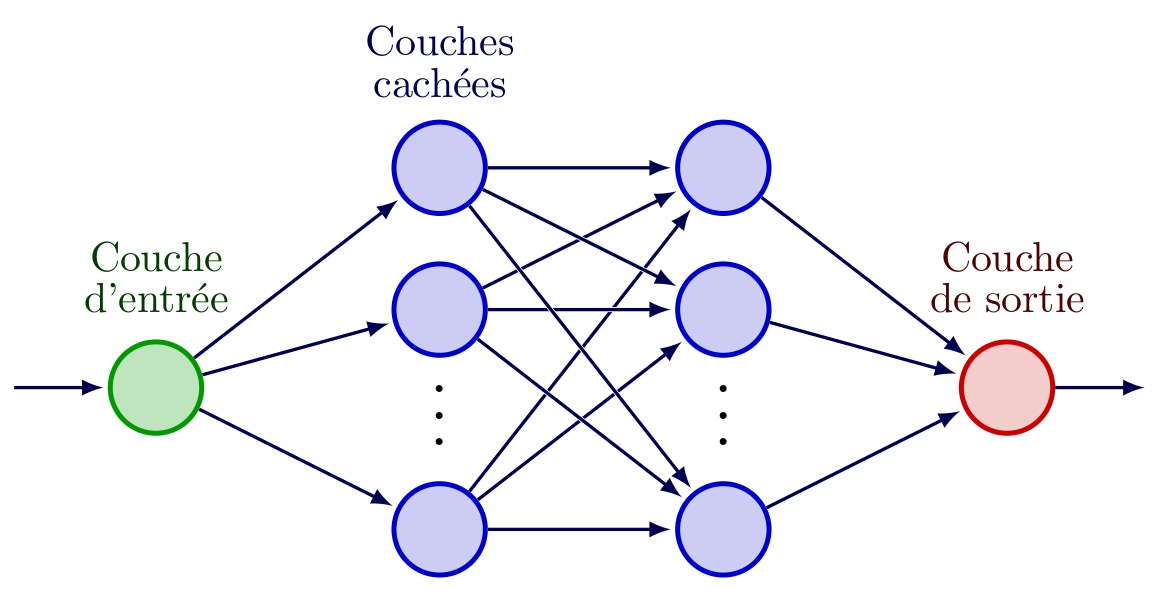
\includegraphics[width = 0.4\textwidth]{FNN/Images/fnnSin/fnnSin_page-0001.jpg}
    \caption[short]{Réseau de neurones pour la fonction $\sin$}
\end{figure}

\begin{figure}[H]
    \centering
    \subfigure[listentry][Données d'entrainement]{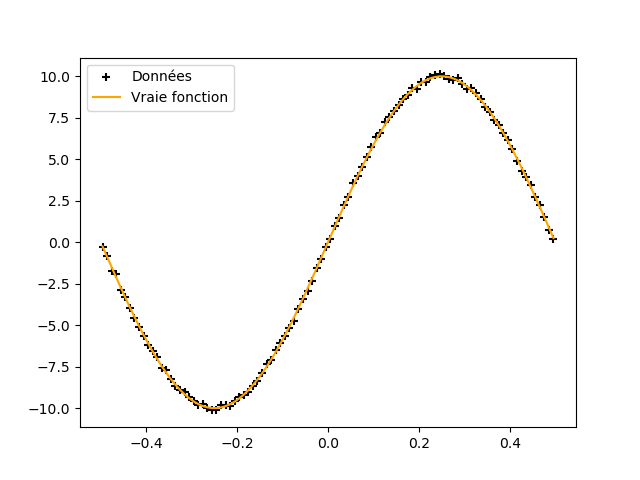
\includegraphics[width = 0.48\textwidth]{../plots/SinPlot.png}}
    \subfigure[listentry][Résultat]{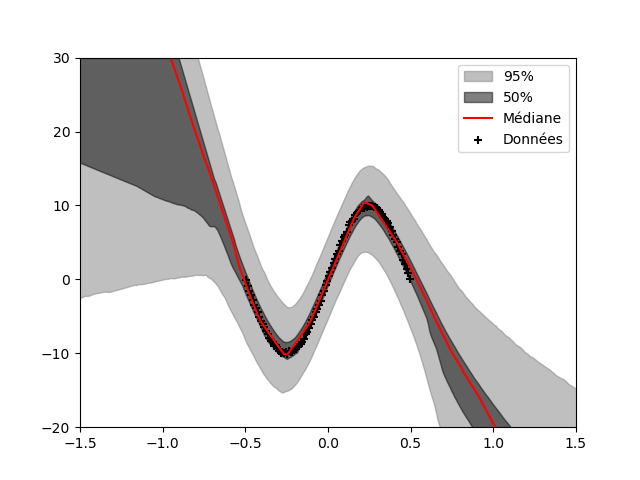
\includegraphics[width = 0.48\textwidth]{../plots/plotSinRes2-12-04-2023_10-48-11.png}}
    \caption[short]{Résultat de l'algorithme BNN-ABC-SS}
\end{figure}

\begin{figure}[H]
    \centering
    \subfigure[]{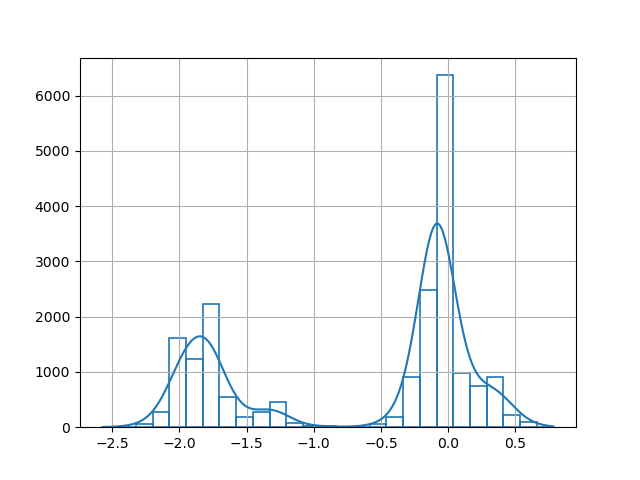
\includegraphics[width = 0.3\textwidth]{../plots/plotWeightSin2-12-04-2023_10-48-11--151.png}}
    \subfigure[]{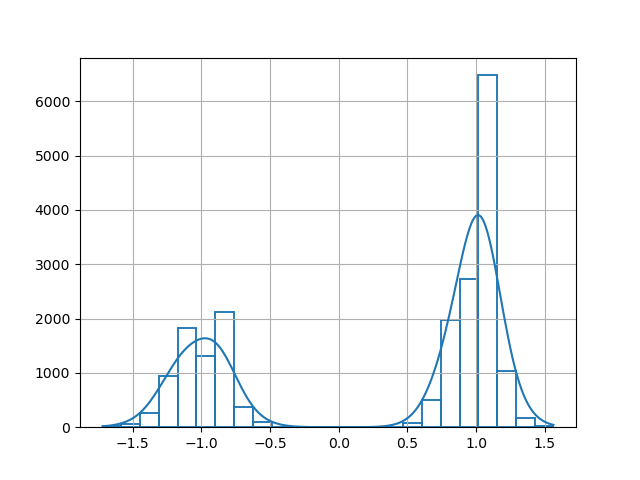
\includegraphics[width = 0.3\textwidth]{../plots/plotWeightSin2-12-04-2023_10-48-11--154.png}}
    \subfigure[]{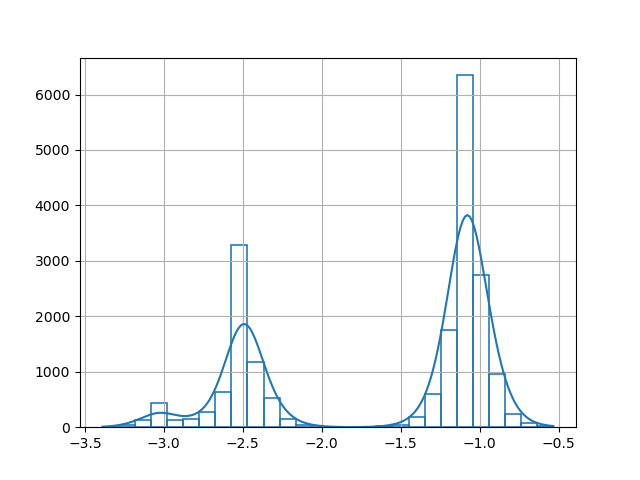
\includegraphics[width = 0.3\textwidth]{../plots/plotWeightSin2-12-04-2023_10-48-11--268.png}}
    \caption[short]{Exemple de distribution a posteriori des poids et biais}
\end{figure}


\begin{figure}[H]
\centering
\begin{tikzpicture}
    \node (img) {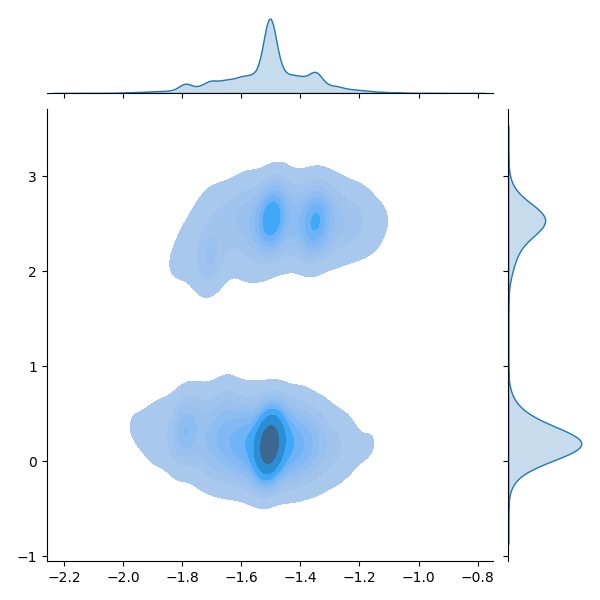
\includegraphics[width = 0.6\textwidth]{../plots/plotWeigthJointSin2-12-04-2023_10-48-11--0&47.png}};
    \node[below=of img, node distance=0cm, yshift=1cm] {$w^{(1)}_{1,1}$};
    \node[left=of img, node distance=0cm, rotate=90, anchor=center,yshift=-0.7cm] {$w^{(2)}_{2,2}$};
\end{tikzpicture}
\caption{Distribution a posteriori de $w^{(1)}_{1,1}$ et $w^{(2)}_{2,2}$}

\end{figure}

\begin{figure}[H]
    \centering
    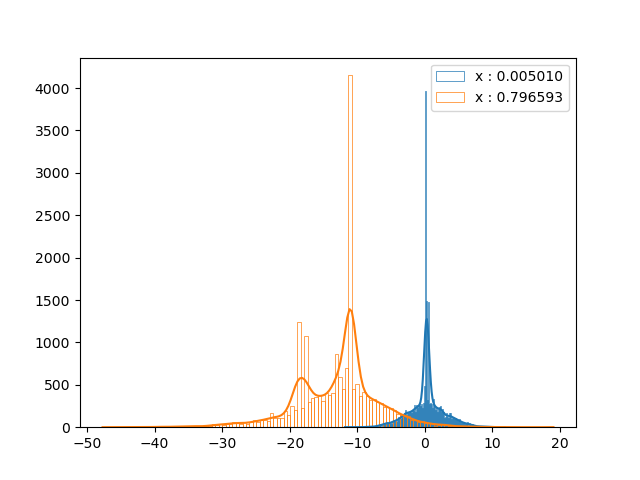
\includegraphics[width = 0.8\textwidth]{../plots/plotIncertitudeSortieSin2-12-04-2023_10-48-11--249&329.png}
    \caption{Distribution sur la sortie pour $x \approx 0$ dans le domaine et et $x \approx 0.8$ hors du domaine}
\end{figure}

\subsection{Maybe more}

Insert im here

list hypperametters

Insert res here


\pagebreak
\section{Conclusion et perspective}
On a vu ici l'implémentation d'une méthode d'approximation sur l'incertitude
sur la sortie qui poura être utilisée par la suite dans ....

\pagebreak
\bibliographystyle{plain}
\bibliography{rapport.bib}

\end{document}
